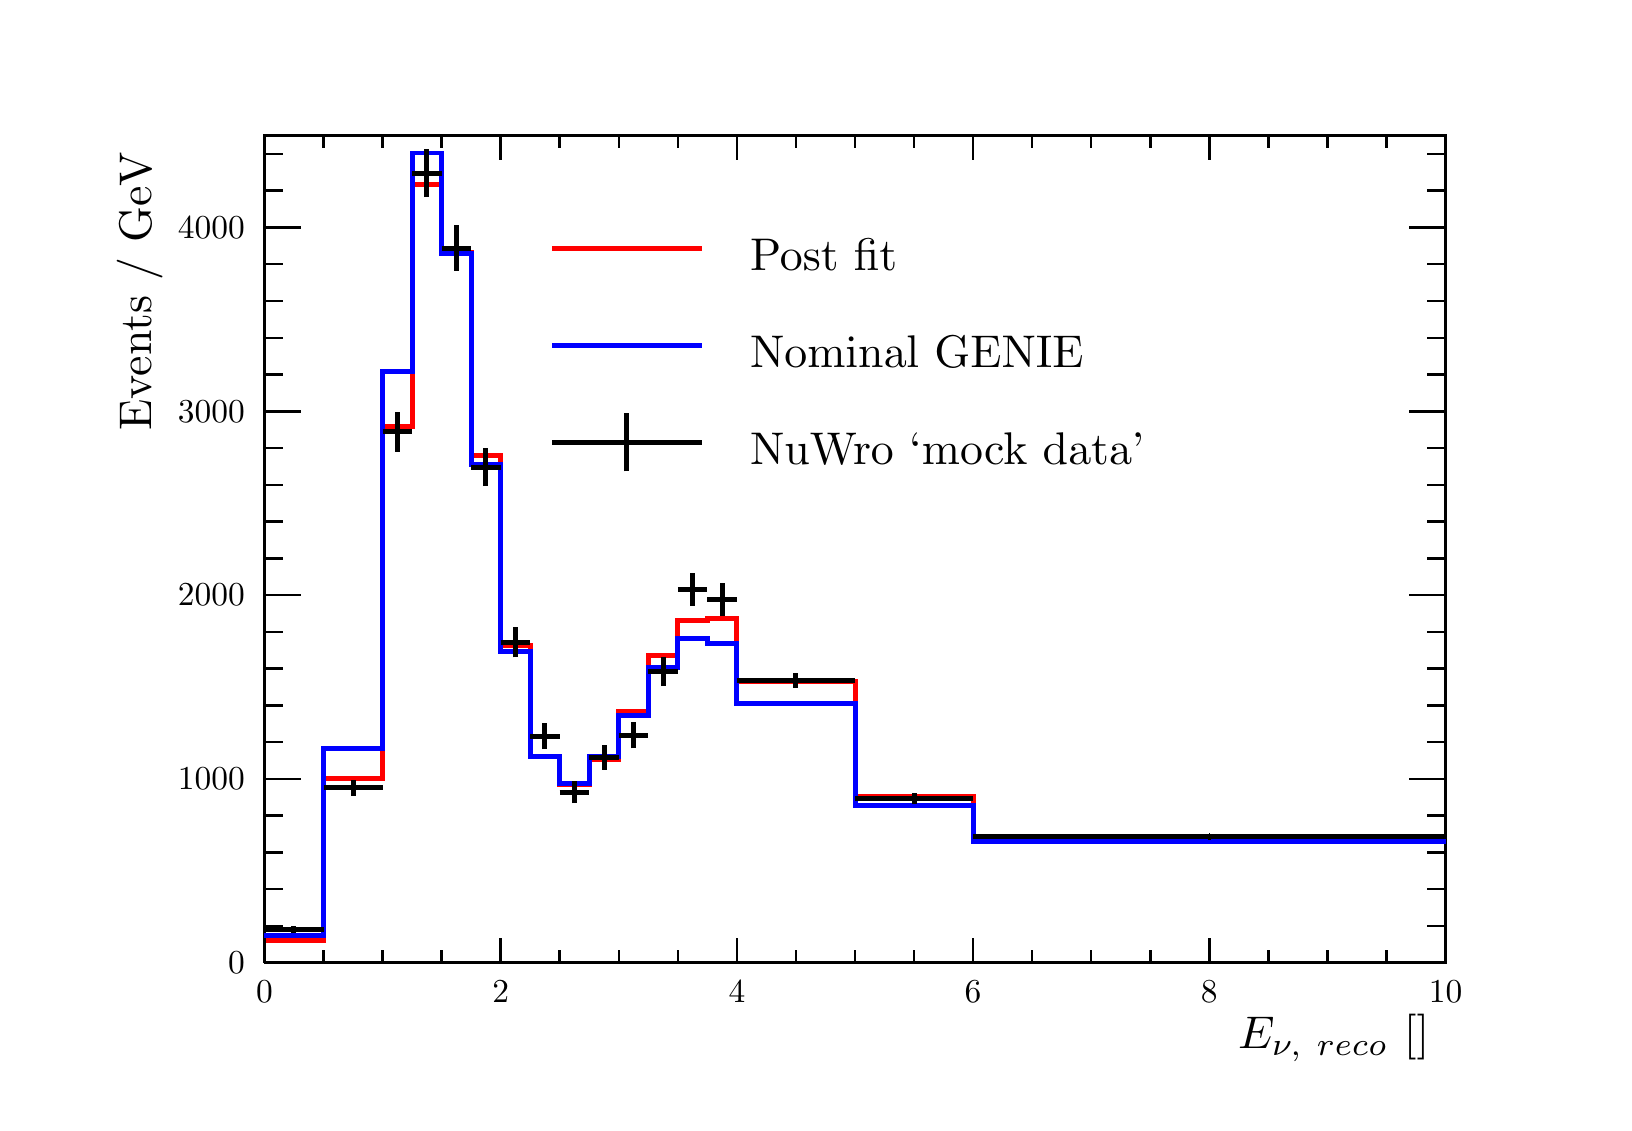
\begin{tikzpicture}
\pgfdeclareplotmark{cross} {
\pgfpathmoveto{\pgfpoint{-0.3\pgfplotmarksize}{\pgfplotmarksize}}
\pgfpathlineto{\pgfpoint{+0.3\pgfplotmarksize}{\pgfplotmarksize}}
\pgfpathlineto{\pgfpoint{+0.3\pgfplotmarksize}{0.3\pgfplotmarksize}}
\pgfpathlineto{\pgfpoint{+1\pgfplotmarksize}{0.3\pgfplotmarksize}}
\pgfpathlineto{\pgfpoint{+1\pgfplotmarksize}{-0.3\pgfplotmarksize}}
\pgfpathlineto{\pgfpoint{+0.3\pgfplotmarksize}{-0.3\pgfplotmarksize}}
\pgfpathlineto{\pgfpoint{+0.3\pgfplotmarksize}{-1.\pgfplotmarksize}}
\pgfpathlineto{\pgfpoint{-0.3\pgfplotmarksize}{-1.\pgfplotmarksize}}
\pgfpathlineto{\pgfpoint{-0.3\pgfplotmarksize}{-0.3\pgfplotmarksize}}
\pgfpathlineto{\pgfpoint{-1.\pgfplotmarksize}{-0.3\pgfplotmarksize}}
\pgfpathlineto{\pgfpoint{-1.\pgfplotmarksize}{0.3\pgfplotmarksize}}
\pgfpathlineto{\pgfpoint{-0.3\pgfplotmarksize}{0.3\pgfplotmarksize}}
\pgfpathclose
\pgfusepathqstroke
}
\pgfdeclareplotmark{cross*} {
\pgfpathmoveto{\pgfpoint{-0.3\pgfplotmarksize}{\pgfplotmarksize}}
\pgfpathlineto{\pgfpoint{+0.3\pgfplotmarksize}{\pgfplotmarksize}}
\pgfpathlineto{\pgfpoint{+0.3\pgfplotmarksize}{0.3\pgfplotmarksize}}
\pgfpathlineto{\pgfpoint{+1\pgfplotmarksize}{0.3\pgfplotmarksize}}
\pgfpathlineto{\pgfpoint{+1\pgfplotmarksize}{-0.3\pgfplotmarksize}}
\pgfpathlineto{\pgfpoint{+0.3\pgfplotmarksize}{-0.3\pgfplotmarksize}}
\pgfpathlineto{\pgfpoint{+0.3\pgfplotmarksize}{-1.\pgfplotmarksize}}
\pgfpathlineto{\pgfpoint{-0.3\pgfplotmarksize}{-1.\pgfplotmarksize}}
\pgfpathlineto{\pgfpoint{-0.3\pgfplotmarksize}{-0.3\pgfplotmarksize}}
\pgfpathlineto{\pgfpoint{-1.\pgfplotmarksize}{-0.3\pgfplotmarksize}}
\pgfpathlineto{\pgfpoint{-1.\pgfplotmarksize}{0.3\pgfplotmarksize}}
\pgfpathlineto{\pgfpoint{-0.3\pgfplotmarksize}{0.3\pgfplotmarksize}}
\pgfpathclose
\pgfusepathqfillstroke
}
\pgfdeclareplotmark{newstar} {
\pgfpathmoveto{\pgfqpoint{0pt}{\pgfplotmarksize}}
\pgfpathlineto{\pgfqpointpolar{44}{0.5\pgfplotmarksize}}
\pgfpathlineto{\pgfqpointpolar{18}{\pgfplotmarksize}}
\pgfpathlineto{\pgfqpointpolar{-20}{0.5\pgfplotmarksize}}
\pgfpathlineto{\pgfqpointpolar{-54}{\pgfplotmarksize}}
\pgfpathlineto{\pgfqpointpolar{-90}{0.5\pgfplotmarksize}}
\pgfpathlineto{\pgfqpointpolar{234}{\pgfplotmarksize}}
\pgfpathlineto{\pgfqpointpolar{198}{0.5\pgfplotmarksize}}
\pgfpathlineto{\pgfqpointpolar{162}{\pgfplotmarksize}}
\pgfpathlineto{\pgfqpointpolar{134}{0.5\pgfplotmarksize}}
\pgfpathclose
\pgfusepathqstroke
}
\pgfdeclareplotmark{newstar*} {
\pgfpathmoveto{\pgfqpoint{0pt}{\pgfplotmarksize}}
\pgfpathlineto{\pgfqpointpolar{44}{0.5\pgfplotmarksize}}
\pgfpathlineto{\pgfqpointpolar{18}{\pgfplotmarksize}}
\pgfpathlineto{\pgfqpointpolar{-20}{0.5\pgfplotmarksize}}
\pgfpathlineto{\pgfqpointpolar{-54}{\pgfplotmarksize}}
\pgfpathlineto{\pgfqpointpolar{-90}{0.5\pgfplotmarksize}}
\pgfpathlineto{\pgfqpointpolar{234}{\pgfplotmarksize}}
\pgfpathlineto{\pgfqpointpolar{198}{0.5\pgfplotmarksize}}
\pgfpathlineto{\pgfqpointpolar{162}{\pgfplotmarksize}}
\pgfpathlineto{\pgfqpointpolar{134}{0.5\pgfplotmarksize}}
\pgfpathclose
\pgfusepathqfillstroke
}
\definecolor{c}{rgb}{1,1,1};
\draw [color=c, fill=c] (0,0) rectangle (20,13.639);
\draw [color=c, fill=c] (3,1.77307) rectangle (18,12.2751);
\definecolor{c}{rgb}{0,0,0};
\draw [c,line width=0.9] (3,1.77307) -- (3,12.2751) -- (18,12.2751) -- (18,1.77307) -- (3,1.77307);
\definecolor{c}{rgb}{1,1,1};
\draw [color=c, fill=c] (3,1.77307) rectangle (18,12.2751);
\definecolor{c}{rgb}{0,0,0};
\draw [c,line width=0.9] (3,1.77307) -- (3,12.2751) -- (18,12.2751) -- (18,1.77307) -- (3,1.77307);
\definecolor{c}{rgb}{1,0,0};
\draw [c,line width=1.8] (3,2.0585) -- (3.75,2.0585) -- (3.75,4.10634) -- (4.5,4.10634) -- (4.5,8.57916) -- (4.875,8.57916) -- (4.875,11.655) -- (5.25,11.655) -- (5.25,10.785) -- (5.625,10.785) -- (5.625,8.21622) -- (6,8.21622) -- (6,5.80071) --
 (6.375,5.80071) -- (6.375,4.38764) -- (6.75,4.38764) -- (6.75,4.0284) -- (7.125,4.0284) -- (7.125,4.35275) -- (7.5,4.35275) -- (7.5,4.96338) -- (7.875,4.96338) -- (7.875,5.66989) -- (8.25,5.66989) -- (8.25,6.117) -- (8.625,6.117) -- (8.625,6.14292)
 -- (9,6.14292) -- (9,5.34375) -- (10.5,5.34375) -- (10.5,3.88265) -- (12,3.88265) -- (12,3.3532) -- (18,3.3532);
\definecolor{c}{rgb}{0,0,0};
\draw [c,line width=0.9] (3,1.77307) -- (18,1.77307);
\draw [c,line width=0.9] (3,2.07994) -- (3,1.77307);
\draw [c,line width=0.9] (3.75,1.9265) -- (3.75,1.77307);
\draw [c,line width=0.9] (4.5,1.9265) -- (4.5,1.77307);
\draw [c,line width=0.9] (5.25,1.9265) -- (5.25,1.77307);
\draw [c,line width=0.9] (6,2.07994) -- (6,1.77307);
\draw [c,line width=0.9] (6.75,1.9265) -- (6.75,1.77307);
\draw [c,line width=0.9] (7.5,1.9265) -- (7.5,1.77307);
\draw [c,line width=0.9] (8.25,1.9265) -- (8.25,1.77307);
\draw [c,line width=0.9] (9,2.07994) -- (9,1.77307);
\draw [c,line width=0.9] (9.75,1.9265) -- (9.75,1.77307);
\draw [c,line width=0.9] (10.5,1.9265) -- (10.5,1.77307);
\draw [c,line width=0.9] (11.25,1.9265) -- (11.25,1.77307);
\draw [c,line width=0.9] (12,2.07994) -- (12,1.77307);
\draw [c,line width=0.9] (12.75,1.9265) -- (12.75,1.77307);
\draw [c,line width=0.9] (13.5,1.9265) -- (13.5,1.77307);
\draw [c,line width=0.9] (14.25,1.9265) -- (14.25,1.77307);
\draw [c,line width=0.9] (15,2.07994) -- (15,1.77307);
\draw [c,line width=0.9] (15.75,1.9265) -- (15.75,1.77307);
\draw [c,line width=0.9] (16.5,1.9265) -- (16.5,1.77307);
\draw [c,line width=0.9] (17.25,1.9265) -- (17.25,1.77307);
\draw [c,line width=0.9] (18,2.07994) -- (18,1.77307);
\draw [anchor=base] (3,1.26842) node[scale=1.20912, color=c, rotate=0]{0};
\draw [anchor=base] (6,1.26842) node[scale=1.20912, color=c, rotate=0]{2};
\draw [anchor=base] (9,1.26842) node[scale=1.20912, color=c, rotate=0]{4};
\draw [anchor=base] (12,1.26842) node[scale=1.20912, color=c, rotate=0]{6};
\draw [anchor=base] (15,1.26842) node[scale=1.20912, color=c, rotate=0]{8};
\draw [anchor=base] (18,1.26842) node[scale=1.20912, color=c, rotate=0]{10};
\draw [anchor= east] (18,0.812882) node[scale=1.65459, color=c, rotate=0]{$E_{\nu,~\text{reco}}$ [\si{\GeV}]};
\draw [c,line width=0.9] (3,12.2751) -- (18,12.2751);
\draw [c,line width=0.9] (3,11.9682) -- (3,12.2751);
\draw [c,line width=0.9] (3.75,12.1216) -- (3.75,12.2751);
\draw [c,line width=0.9] (4.5,12.1216) -- (4.5,12.2751);
\draw [c,line width=0.9] (5.25,12.1216) -- (5.25,12.2751);
\draw [c,line width=0.9] (6,11.9682) -- (6,12.2751);
\draw [c,line width=0.9] (6.75,12.1216) -- (6.75,12.2751);
\draw [c,line width=0.9] (7.5,12.1216) -- (7.5,12.2751);
\draw [c,line width=0.9] (8.25,12.1216) -- (8.25,12.2751);
\draw [c,line width=0.9] (9,11.9682) -- (9,12.2751);
\draw [c,line width=0.9] (9.75,12.1216) -- (9.75,12.2751);
\draw [c,line width=0.9] (10.5,12.1216) -- (10.5,12.2751);
\draw [c,line width=0.9] (11.25,12.1216) -- (11.25,12.2751);
\draw [c,line width=0.9] (12,11.9682) -- (12,12.2751);
\draw [c,line width=0.9] (12.75,12.1216) -- (12.75,12.2751);
\draw [c,line width=0.9] (13.5,12.1216) -- (13.5,12.2751);
\draw [c,line width=0.9] (14.25,12.1216) -- (14.25,12.2751);
\draw [c,line width=0.9] (15,11.9682) -- (15,12.2751);
\draw [c,line width=0.9] (15.75,12.1216) -- (15.75,12.2751);
\draw [c,line width=0.9] (16.5,12.1216) -- (16.5,12.2751);
\draw [c,line width=0.9] (17.25,12.1216) -- (17.25,12.2751);
\draw [c,line width=0.9] (18,11.9682) -- (18,12.2751);
\draw [c,line width=0.9] (3,1.77307) -- (3,12.2751);
\draw [c,line width=0.9] (3.462,1.77307) -- (3,1.77307);
\draw [c,line width=0.9] (3.231,2.23982) -- (3,2.23982);
\draw [c,line width=0.9] (3.231,2.70658) -- (3,2.70658);
\draw [c,line width=0.9] (3.231,3.17333) -- (3,3.17333);
\draw [c,line width=0.9] (3.231,3.64009) -- (3,3.64009);
\draw [c,line width=0.9] (3.462,4.10684) -- (3,4.10684);
\draw [c,line width=0.9] (3.231,4.5736) -- (3,4.5736);
\draw [c,line width=0.9] (3.231,5.04036) -- (3,5.04036);
\draw [c,line width=0.9] (3.231,5.50711) -- (3,5.50711);
\draw [c,line width=0.9] (3.231,5.97387) -- (3,5.97387);
\draw [c,line width=0.9] (3.462,6.44062) -- (3,6.44062);
\draw [c,line width=0.9] (3.231,6.90738) -- (3,6.90738);
\draw [c,line width=0.9] (3.231,7.37414) -- (3,7.37414);
\draw [c,line width=0.9] (3.231,7.84089) -- (3,7.84089);
\draw [c,line width=0.9] (3.231,8.30765) -- (3,8.30765);
\draw [c,line width=0.9] (3.462,8.7744) -- (3,8.7744);
\draw [c,line width=0.9] (3.231,9.24116) -- (3,9.24116);
\draw [c,line width=0.9] (3.231,9.70791) -- (3,9.70791);
\draw [c,line width=0.9] (3.231,10.1747) -- (3,10.1747);
\draw [c,line width=0.9] (3.231,10.6414) -- (3,10.6414);
\draw [c,line width=0.9] (3.462,11.1082) -- (3,11.1082);
\draw [c,line width=0.9] (3.462,11.1082) -- (3,11.1082);
\draw [c,line width=0.9] (3.231,11.5749) -- (3,11.5749);
\draw [c,line width=0.9] (3.231,12.0417) -- (3,12.0417);
\draw [anchor= east] (2.9,1.77307) node[scale=1.20912, color=c, rotate=0]{0};
\draw [anchor= east] (2.9,4.10684) node[scale=1.20912, color=c, rotate=0]{1000};
\draw [anchor= east] (2.9,6.44062) node[scale=1.20912, color=c, rotate=0]{2000};
\draw [anchor= east] (2.9,8.7744) node[scale=1.20912, color=c, rotate=0]{3000};
\draw [anchor= east] (2.9,11.1082) node[scale=1.20912, color=c, rotate=0]{4000};
\draw [anchor= east] (1.416,12.2751) node[scale=1.65459, color=c, rotate=90]{Events / GeV};
\draw [c,line width=0.9] (18,1.77307) -- (18,12.2751);
\draw [c,line width=0.9] (17.538,1.77307) -- (18,1.77307);
\draw [c,line width=0.9] (17.769,2.23982) -- (18,2.23982);
\draw [c,line width=0.9] (17.769,2.70658) -- (18,2.70658);
\draw [c,line width=0.9] (17.769,3.17333) -- (18,3.17333);
\draw [c,line width=0.9] (17.769,3.64009) -- (18,3.64009);
\draw [c,line width=0.9] (17.538,4.10684) -- (18,4.10684);
\draw [c,line width=0.9] (17.769,4.5736) -- (18,4.5736);
\draw [c,line width=0.9] (17.769,5.04036) -- (18,5.04036);
\draw [c,line width=0.9] (17.769,5.50711) -- (18,5.50711);
\draw [c,line width=0.9] (17.769,5.97387) -- (18,5.97387);
\draw [c,line width=0.9] (17.538,6.44062) -- (18,6.44062);
\draw [c,line width=0.9] (17.769,6.90738) -- (18,6.90738);
\draw [c,line width=0.9] (17.769,7.37414) -- (18,7.37414);
\draw [c,line width=0.9] (17.769,7.84089) -- (18,7.84089);
\draw [c,line width=0.9] (17.769,8.30765) -- (18,8.30765);
\draw [c,line width=0.9] (17.538,8.7744) -- (18,8.7744);
\draw [c,line width=0.9] (17.769,9.24116) -- (18,9.24116);
\draw [c,line width=0.9] (17.769,9.70791) -- (18,9.70791);
\draw [c,line width=0.9] (17.769,10.1747) -- (18,10.1747);
\draw [c,line width=0.9] (17.769,10.6414) -- (18,10.6414);
\draw [c,line width=0.9] (17.538,11.1082) -- (18,11.1082);
\draw [c,line width=0.9] (17.538,11.1082) -- (18,11.1082);
\draw [c,line width=0.9] (17.769,11.5749) -- (18,11.5749);
\draw [c,line width=0.9] (17.769,12.0417) -- (18,12.0417);
\definecolor{c}{rgb}{0,0,1};
\draw [c,line width=1.8] (3,2.11511) -- (3.75,2.11511) -- (3.75,4.48663) -- (4.5,4.48663) -- (4.5,9.27454) -- (4.875,9.27454) -- (4.875,12.0542) -- (5.25,12.0542) -- (5.25,10.7771) -- (5.625,10.7771) -- (5.625,8.09622) -- (6,8.09622) -- (6,5.71841)
 -- (6.375,5.71841) -- (6.375,4.39589) -- (6.75,4.39589) -- (6.75,4.05305) -- (7.125,4.05305) -- (7.125,4.38483) -- (7.5,4.38483) -- (7.5,4.91355) -- (7.875,4.91355) -- (7.875,5.51564) -- (8.25,5.51564) -- (8.25,5.8905) -- (8.625,5.8905) --
 (8.625,5.82701) -- (9,5.82701) -- (9,5.06382) -- (10.5,5.06382) -- (10.5,3.76265) -- (12,3.76265) -- (12,3.30444) -- (18,3.30444);
\definecolor{c}{rgb}{0,0,0};
\draw [c,line width=1.8] (3.375,2.14444) -- (3.375,2.18848);
\draw [c,line width=1.8] (3.375,2.18848) -- (3.375,2.23251);
\draw [c,line width=1.8] (3,2.18848) -- (3.375,2.18848);
\draw [c,line width=1.8] (3.375,2.18848) -- (3.75,2.18848);
\foreach \P in {(3.375,2.18848)}{\draw[mark options={color=c,fill=c},mark size=2.402402pt, line width=0.000000pt, mark=*,mark size=1pt] plot coordinates {\P};}
\draw [c,line width=1.8] (4.125,3.89299) -- (4.125,3.99482);
\draw [c,line width=1.8] (4.125,3.99482) -- (4.125,4.09666);
\draw [c,line width=1.8] (3.75,3.99482) -- (4.125,3.99482);
\draw [c,line width=1.8] (4.125,3.99482) -- (4.5,3.99482);
\foreach \P in {(4.125,3.99482)}{\draw[mark options={color=c,fill=c},mark size=2.402402pt, line width=0.000000pt, mark=*,mark size=1pt] plot coordinates {\P};}
\draw [c,line width=1.8] (4.6875,8.26219) -- (4.6875,8.51302);
\draw [c,line width=1.8] (4.6875,8.51302) -- (4.6875,8.76385);
\draw [c,line width=1.8] (4.5,8.51302) -- (4.6875,8.51302);
\draw [c,line width=1.8] (4.6875,8.51302) -- (4.875,8.51302);
\foreach \P in {(4.6875,8.51302)}{\draw[mark options={color=c,fill=c},mark size=2.402402pt, line width=0.000000pt, mark=*,mark size=1pt] plot coordinates {\P};}
\draw [c,line width=1.8] (5.0625,11.4931) -- (5.0625,11.799);
\draw [c,line width=1.8] (5.0625,11.799) -- (5.0625,12.1049);
\draw [c,line width=1.8] (4.875,11.799) -- (5.0625,11.799);
\draw [c,line width=1.8] (5.0625,11.799) -- (5.25,11.799);
\foreach \P in {(5.0625,11.799)}{\draw[mark options={color=c,fill=c},mark size=2.402402pt, line width=0.000000pt, mark=*,mark size=1pt] plot coordinates {\P};}
\draw [c,line width=1.8] (5.4375,10.5558) -- (5.4375,10.8468);
\draw [c,line width=1.8] (5.4375,10.8468) -- (5.4375,11.1378);
\draw [c,line width=1.8] (5.25,10.8468) -- (5.4375,10.8468);
\draw [c,line width=1.8] (5.4375,10.8468) -- (5.625,10.8468);
\foreach \P in {(5.4375,10.8468)}{\draw[mark options={color=c,fill=c},mark size=2.402402pt, line width=0.000000pt, mark=*,mark size=1pt] plot coordinates {\P};}
\draw [c,line width=1.8] (5.8125,7.82258) -- (5.8125,8.06493);
\draw [c,line width=1.8] (5.8125,8.06493) -- (5.8125,8.30729);
\draw [c,line width=1.8] (5.625,8.06493) -- (5.8125,8.06493);
\draw [c,line width=1.8] (5.8125,8.06493) -- (6,8.06493);
\foreach \P in {(5.8125,8.06493)}{\draw[mark options={color=c,fill=c},mark size=2.402402pt, line width=0.000000pt, mark=*,mark size=1pt] plot coordinates {\P};}
\draw [c,line width=1.8] (6.1875,5.64825) -- (6.1875,5.84318);
\draw [c,line width=1.8] (6.1875,5.84318) -- (6.1875,6.0381);
\draw [c,line width=1.8] (6,5.84318) -- (6.1875,5.84318);
\draw [c,line width=1.8] (6.1875,5.84318) -- (6.375,5.84318);
\foreach \P in {(6.1875,5.84318)}{\draw[mark options={color=c,fill=c},mark size=2.402402pt, line width=0.000000pt, mark=*,mark size=1pt] plot coordinates {\P};}
\draw [c,line width=1.8] (6.5625,4.48445) -- (6.5625,4.64828);
\draw [c,line width=1.8] (6.5625,4.64828) -- (6.5625,4.81211);
\draw [c,line width=1.8] (6.375,4.64828) -- (6.5625,4.64828);
\draw [c,line width=1.8] (6.5625,4.64828) -- (6.75,4.64828);
\foreach \P in {(6.5625,4.64828)}{\draw[mark options={color=c,fill=c},mark size=2.402402pt, line width=0.000000pt, mark=*,mark size=1pt] plot coordinates {\P};}
\draw [c,line width=1.8] (6.9375,3.79662) -- (6.9375,3.93881);
\draw [c,line width=1.8] (6.9375,3.93881) -- (6.9375,4.081);
\draw [c,line width=1.8] (6.75,3.93881) -- (6.9375,3.93881);
\draw [c,line width=1.8] (6.9375,3.93881) -- (7.125,3.93881);
\foreach \P in {(6.9375,3.93881)}{\draw[mark options={color=c,fill=c},mark size=2.402402pt, line width=0.000000pt, mark=*,mark size=1pt] plot coordinates {\P};}
\draw [c,line width=1.8] (7.3125,4.22164) -- (7.3125,4.37756);
\draw [c,line width=1.8] (7.3125,4.37756) -- (7.3125,4.53349);
\draw [c,line width=1.8] (7.125,4.37756) -- (7.3125,4.37756);
\draw [c,line width=1.8] (7.3125,4.37756) -- (7.5,4.37756);
\foreach \P in {(7.3125,4.37756)}{\draw[mark options={color=c,fill=c},mark size=2.402402pt, line width=0.000000pt, mark=*,mark size=1pt] plot coordinates {\P};}
\draw [c,line width=1.8] (7.6875,4.49352) -- (7.6875,4.65762);
\draw [c,line width=1.8] (7.6875,4.65762) -- (7.6875,4.82171);
\draw [c,line width=1.8] (7.5,4.65762) -- (7.6875,4.65762);
\draw [c,line width=1.8] (7.6875,4.65762) -- (7.875,4.65762);
\foreach \P in {(7.6875,4.65762)}{\draw[mark options={color=c,fill=c},mark size=2.402402pt, line width=0.000000pt, mark=*,mark size=1pt] plot coordinates {\P};}
\draw [c,line width=1.8] (8.0625,5.28401) -- (8.0625,5.46977);
\draw [c,line width=1.8] (8.0625,5.46977) -- (8.0625,5.65554);
\draw [c,line width=1.8] (7.875,5.46977) -- (8.0625,5.46977);
\draw [c,line width=1.8] (8.0625,5.46977) -- (8.25,5.46977);
\foreach \P in {(8.0625,5.46977)}{\draw[mark options={color=c,fill=c},mark size=2.402402pt, line width=0.000000pt, mark=*,mark size=1pt] plot coordinates {\P};}
\draw [c,line width=1.8] (8.4375,6.3049) -- (8.4375,6.51531);
\draw [c,line width=1.8] (8.4375,6.51531) -- (8.4375,6.72571);
\draw [c,line width=1.8] (8.25,6.51531) -- (8.4375,6.51531);
\draw [c,line width=1.8] (8.4375,6.51531) -- (8.625,6.51531);
\foreach \P in {(8.4375,6.51531)}{\draw[mark options={color=c,fill=c},mark size=2.402402pt, line width=0.000000pt, mark=*,mark size=1pt] plot coordinates {\P};}
\draw [c,line width=1.8] (8.8125,6.17713) -- (8.8125,6.38461);
\draw [c,line width=1.8] (8.8125,6.38461) -- (8.8125,6.5921);
\draw [c,line width=1.8] (8.625,6.38461) -- (8.8125,6.38461);
\draw [c,line width=1.8] (8.8125,6.38461) -- (9,6.38461);
\foreach \P in {(8.8125,6.38461)}{\draw[mark options={color=c,fill=c},mark size=2.402402pt, line width=0.000000pt, mark=*,mark size=1pt] plot coordinates {\P};}
\draw [c,line width=1.8] (9.75,5.26168) -- (9.75,5.35308);
\draw [c,line width=1.8] (9.75,5.35308) -- (9.75,5.44449);
\draw [c,line width=1.8] (9,5.35308) -- (9.75,5.35308);
\draw [c,line width=1.8] (9.75,5.35308) -- (10.5,5.35308);
\foreach \P in {(9.75,5.35308)}{\draw[mark options={color=c,fill=c},mark size=2.402402pt, line width=0.000000pt, mark=*,mark size=1pt] plot coordinates {\P};}
\draw [c,line width=1.8] (11.25,3.78968) -- (11.25,3.85946);
\draw [c,line width=1.8] (11.25,3.85946) -- (11.25,3.92924);
\draw [c,line width=1.8] (10.5,3.85946) -- (11.25,3.85946);
\draw [c,line width=1.8] (11.25,3.85946) -- (12,3.85946);
\foreach \P in {(11.25,3.85946)}{\draw[mark options={color=c,fill=c},mark size=2.402402pt, line width=0.000000pt, mark=*,mark size=1pt] plot coordinates {\P};}
\draw [c,line width=1.8] (15,3.34059) -- (15,3.37112);
\draw [c,line width=1.8] (15,3.37112) -- (15,3.40166);
\draw [c,line width=1.8] (12,3.37112) -- (15,3.37112);
\draw [c,line width=1.8] (15,3.37112) -- (18,3.37112);
\foreach \P in {(15,3.37112)}{\draw[mark options={color=c,fill=c},mark size=2.402402pt, line width=0.000000pt, mark=*,mark size=1pt] plot coordinates {\P};}
\definecolor{c}{rgb}{1,1,1};
\draw [color=c, fill=c] (2,12.8206) rectangle (18,13.5708);
\definecolor{c}{rgb}{0,0,0};
%\draw (10,13.1957) node[scale=1.40004, color=c, rotate=0]{$\nu_{\mu} FHC postfit: \delta = 1.57, \chi^{2} = 51.36$};
\definecolor{c}{rgb}{1,1,1};
\draw [color=c, fill=c] (6.24642,7.76504) rectangle (17.106,11.4613);
\definecolor{c}{rgb}{0,0,0};
\draw [anchor=base west] (8.96132,10.5681) node[scale=1.65459, color=c, rotate=0]{Post fit};
\definecolor{c}{rgb}{1,0,0};
\draw [c,line width=1.8] (6.65365,10.8453) -- (8.55408,10.8453);
\definecolor{c}{rgb}{0,0,0};
\draw [anchor=base west] (8.96132,9.33596) node[scale=1.65459, color=c, rotate=0]{Nominal GENIE};
\definecolor{c}{rgb}{0,0,1};
\draw [c,line width=1.8] (6.65365,9.61318) -- (8.55408,9.61318);
\definecolor{c}{rgb}{0,0,0};
\draw [anchor=base west] (8.96132,8.10387) node[scale=1.65459, color=c, rotate=0]{NuWro `mock data'};
\draw [c,line width=1.8] (6.65365,8.38109) -- (8.55408,8.38109);
\draw [c,line width=1.8] (7.60387,8.01146) -- (7.60387,8.75072);
\end{tikzpicture}
